\section{Timer \& Event Counters \refskript{7.4}}
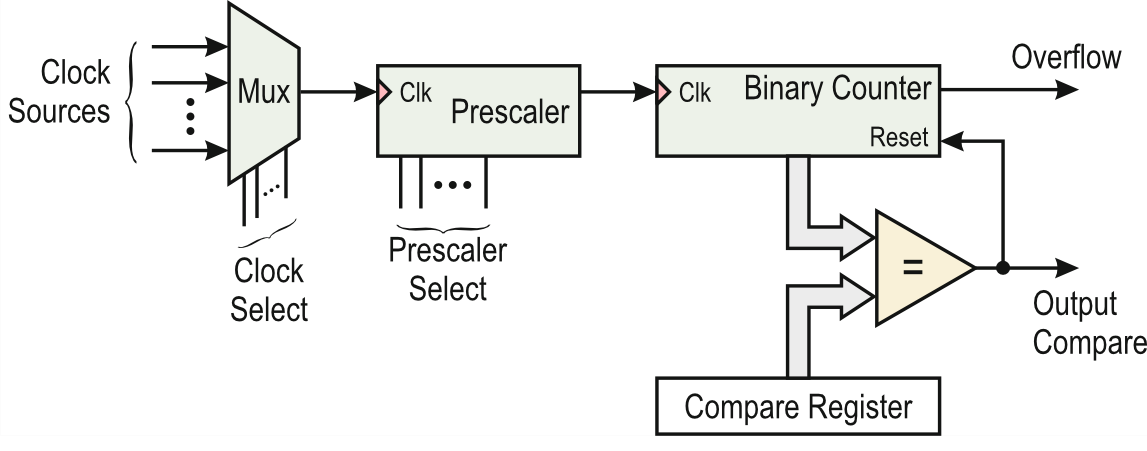
\includegraphics[width=\columnwidth]{"Images/TimerFuntionsweise.png"}
\begin{lstlisting}[language=C]
//************ TimerB0 configuration ************//
TB0CTL |= 0x0004;   //clear timer (set TBCLR Bit)
TB0CTL |= 0x0200;   //select SMCLK as inputClock
TB0CCR0 = period;   //set period
TB0CCTL2 = 0x00E0;  //set Output-Mode to Reset/Set
TB0CCR2 = 0x0000;   //set a default duty cycle value
\end{lstlisting}\vspace{-20px}


\formula{$\text{Compare Register} = \text{cnt} \div \text{prescaler} - 1$}

\subsection{Signature Timer Applications \refskript{7.4.3}}
\textit{Watchdog timer} is secured through a password in the \textit{WDTCTL} register.
\textit{Real-Time Clocks} provides absolute time (second, minute, hour, day, month, week).
\textit{Baud Rate Generation} can provide clock base for baud rate.

\begin{minipage}{.5\columnwidth}
	\formula{$\mathit{baudrate} = \dfrac{f_{\mathit{clk}}}{\mathit{PS} \cdot \mathit{TopCount}}$}
\end{minipage}
\begin{minipage}{.5\columnwidth}
	\unitText{$\mathit{PS}$}{Prescale Factor}{1}\\
	\unitText{$f_{\mathit{clk}}$}{Clock frequency}{Hz}\\
	\unitText{$\mathit{TopCount}$}{Compare value}{1}
\end{minipage}

\subsubsection{MSP430 Timer Support \refskript{7.4.4}}

Operating Modes

Input Capture Operation

Measuring a Signal Width

Output Compare Operation
